\documentclass{article}

% Use final NeurIPS (two-column)
\usepackage[final]{neurips_2022}

% Basics
\usepackage[utf8]{inputenc}
\usepackage[T1]{fontenc}
\usepackage{microtype}
\usepackage{hyperref}
\usepackage{url}
\usepackage{amsmath,amssymb}
\usepackage{booktabs}
\usepackage{xcolor}
% Algorithm package - using algorithm2e for better compatibility
\usepackage[ruled,vlined,linesnumbered]{algorithm2e}


% Floats/graphics
\usepackage{caption}
\captionsetup{font=small}
\setlength{\textfloatsep}{6pt plus 2pt minus 2pt}
\setlength{\abovecaptionskip}{3pt}
\setlength{\belowcaptionskip}{0pt}

\usepackage{tikz}
\usetikzlibrary{positioning,arrows.meta}

\title{Project Milestone --- Literature Review:\\ A Dual--SPMA Framework for Convex MDPs}

\author{
Shervin Khamooshian \quad Ahmed Magd \quad Pegah Aryadoost \quad Danielle Nguyen\\
Simon Fraser University \qquad \texttt{\{ska309, ams80, paa40, tdSn8\}@sfu.ca}
}

\begin{document}
\maketitle

\section*{Project topic (what we are building)}
\textbf{Goal.} We study a unified way to solve \emph{Convex MDPs (CMDPs)} by combining a Fenchel-dual saddle formulation with a geometry-aware policy optimizer, \emph{Softmax Policy Mirror Ascent (SPMA)}. CMDPs minimize a convex function of discounted occupancies and are equivalent to the saddle
$\min_{\pi}\max_{y}\ \langle y,d_{\pi}\rangle-f^*(y)$. Fixing $y$ turns the policy step into standard RL with shaped reward $r_y(s,a)=-y(s,a)$ (or $-\,\phi(s,a)^\top y$ under features). We alternate a mirror-ascent step on $y$ with an SPMA policy step and return discounted occupancy (or feature-expectation) estimates for the next dual update (Fig.~\ref{fig:dualspma}).

\begin{figure}[t]
\centering
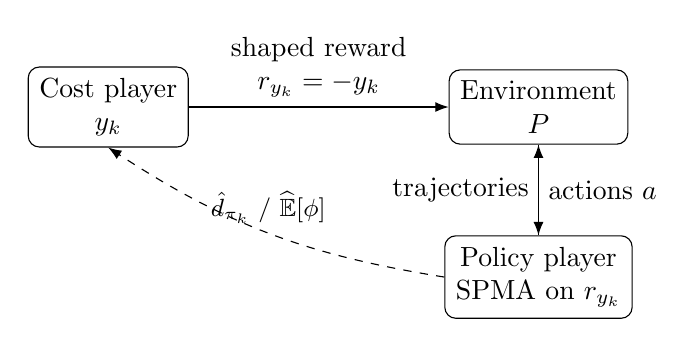
\begin{tikzpicture}[node distance=1.55cm, >=Latex]
\node[draw, rounded corners, align=center, inner sep=4pt] (cost) {Cost player\\$y_k$};
\node[draw, rounded corners, align=center, inner sep=4pt, right=3.3cm of cost] (env) {Environment\\$P$};
\node[draw, rounded corners, align=center, inner sep=4pt, below=1.15cm of env] (policy) {Policy player\\SPMA on $r_{y_k}$};
\draw[->] (cost) -- node[above, align=center]{shaped reward\\$r_{y_k}=-y_k$} (env);
\draw[->] (policy) -- node[right]{actions $a$} (env);
\draw[->] (env) -- node[left]{trajectories} (policy);
\draw[->, dashed, bend left=12] (policy.west) to node[above]{\small $\hat d_{\pi_k}$ / $\widehat{\mathbb E}[\phi]$} (cost.south);
\end{tikzpicture}
\caption{\textbf{Dual--SPMA loop.} Dual ascent chooses $y_k$, which induces a shaped reward for the SPMA policy step; discounted occupancies feed the next dual update.}
\label{fig:dualspma}
\end{figure}


% =================== Paper 1 ====================================
\section*{Paper 1: \emph{Reward is Enough for Convex MDPs} (NeurIPS 2021)}
\textbf{Core idea.} Many RL goals can be posed as $\min_{d\in\mathcal{K}} f(d)$ for convex $f$ over the occupancy polytope $\mathcal{K}$. Using Fenchel conjugacy,
\(
\min_{d\in \mathcal{K}} f(d)=\min_{d\in \mathcal{K}}\max_{\lambda\in\Lambda}\ \lambda\!\cdot\! d - f^*(\lambda),
\)
so for fixed $\lambda$ the policy subproblem is vanilla RL with shaped reward $r_\lambda=-\lambda$. 

\begin{figure}[h]
\centering
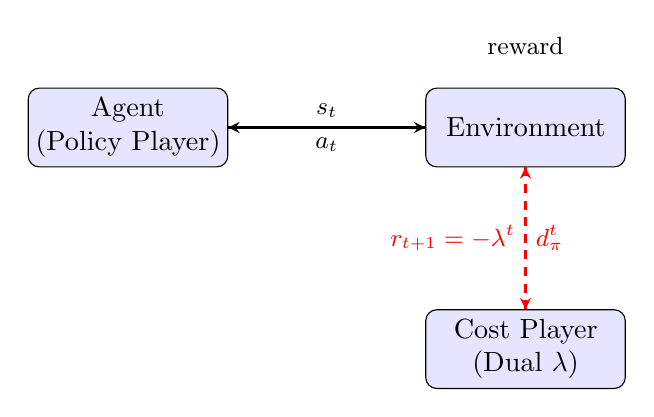
\begin{tikzpicture}[
    node distance=2.5cm,
    block/.style={rectangle, draw, fill=blue!10, text width=2.3cm, text centered, 
                  minimum height=1cm, rounded corners},
    arrow/.style={->, >=stealth, thick}
]
\node[block] (agent) {Agent\\(Policy Player)};
\node[block, right=of agent] (env) {Environment};
\node[block, below=1.8cm of env] (cost) {Cost Player\\(Dual $\lambda$)};
\draw[arrow] (env) -- node[above, font=\small] {$s_t$} (agent);
\draw[arrow] (agent) -- node[below, font=\small] {$a_t$} (env);
\draw[arrow, dashed, red, thick] (cost) -- node[left, font=\small] {$r_{t+1} = -\lambda^t$} (env);
\draw[arrow, dashed, red, thick] (env) -- node[right, font=\small] {$d_\pi^t$} (cost);
\node[above=0.3cm of env, font=\small] {reward};
\end{tikzpicture}
\caption{Convex MDP as a two-player game (adapted from \citet{zahavy2021reward}, Fig.~1). 
The cost player provides non-stationary shaped rewards $r_t = -\lambda^t$ to the agent, 
observing the resulting occupancy measures $d_\pi^t$. From the agent's perspective, this 
reduces to standard RL with time-varying rewards.}
\label{fig:convex_mdp_game}
\end{figure}

Figure~\ref{fig:convex_mdp_game} illustrates this as a two-player game where the agent sees non-stationary rewards from the cost player. A meta-algorithm (Algorithm~\ref{alg:convex_mdp_meta}) alternates a \emph{cost player} (FTL/OMD in $\lambda$, a convex ascent step) with a \emph{policy player} (best response or low-regret RL, which reduces to ``just RL'' under the shaped reward), yielding $O(1/\sqrt{K})$ optimization error for averaged iterates under standard OCO assumptions. The paper shows best-response is ideal but often intractable in deep RL, so low-regret learners (e.g., UCRL2, MDPO) suffice; the guarantees hold for averaged occupancies $\bar{d}_\pi^K$ rather than single iterates. It unifies apprenticeship learning, CMDPs and pure exploration (Table~\ref{tab:convex_mdp_examples}). \citep{zahavy2021reward}


% Algorithm using algorithm2e syntax
\begin{algorithm}[h]
\caption{Meta-algorithm for Convex MDPs \citep{zahavy2021reward}}
\label{alg:convex_mdp_meta}
\small
\KwIn{Convex-concave payoff $\mathcal{L}: \mathcal{K} \times \Lambda \to \mathbb{R}$, algorithms $\text{Alg}_\lambda$, $\text{Alg}_\pi$, $K \in \mathbb{N}$}
\For{$k = 1, \ldots, K$}{
    $\lambda^k \leftarrow \text{Alg}_\lambda(d_\pi^1, \ldots, d_\pi^{k-1}; \mathcal{L})$ \tcp*{Cost player update}
    $d_\pi^k \leftarrow \text{Alg}_\pi(-\lambda^k)$ \tcp*{Policy: solve RL with $r = -\lambda^k$}
}
\KwOut{$\bar{d}_\pi^K = \frac{1}{K}\sum_{k=1}^K d_\pi^k$, $\bar{\lambda}^K = \frac{1}{K}\sum_{k=1}^K \lambda^k$}
\end{algorithm}


\textbf{Relevance.} This work justifies the saddle and the shaped-reward reduction we implement and informs our outer-loop design (dual MA + policy best response).

% =================== Paper 2 ====================================
\section*{Paper 2: \emph{Fast Convergence of Softmax Policy Mirror Ascent} (OPT 2024 / arXiv 2025)}
\textbf{Core idea.} \emph{SPMA} performs mirror ascent in \emph{logit} space using the log-sum-exp mirror map, in contrast to NPG which uses exponential reweighting in probability space (Sec.~3.2). In tabular MDPs the per-state update (Eq.~3)
$\pi_{t+1}(a|s)=\pi_t(a|s)\bigl(1+\eta\,A^{\pi_t}(s,a)\bigr)$
avoids explicit normalization and achieves \emph{linear convergence} for sufficiently small constant step-size: bandit linear convergence (Thm.~1) and tabular MDP linear convergence to the optimal value (Thm.~2), improving over softmax PG (Sec.~3.3). For large problems, SPMA projects onto function classes via convex \emph{softmax classification} subproblems (Eq.~4--5, Algorithm~1) and proves linear convergence to a neighbourhood under FA (Sec.~4); the theory assumes exact or low-noise gradients, and performance depends on advantage-estimation quality (Sec.~4.2). Empirically it competes with PPO/TRPO/MDPO (Sec.~4.1). \citep{asad2024fast}

\textbf{Relevance.} We need a strong policy ``best response'' in Zahavy's saddle; SPMA provides the geometry and fast rates in tabular settings, plus a practical FA implementation (convex surrogates that fit deep RL) matching our shaped-reward reduction.

% =================== Paper 3 ====================================
\section*{Paper 3: \emph{Natural Policy Gradient Primal--Dual for CMDPs} (NeurIPS 2020)}
\textbf{Core idea.} A policy-based primal--dual method for the Lagrangian CMDP formulation $V_r^\pi(\rho)+\lambda(V_g^\pi(\rho)-b)$: \emph{natural policy gradient} (NPG) ascent for the policy and projected subgradient updates for the multiplier (Eq.~7--8, Sec.~3--4), showing a multiplicative update for softmax policies and projection for $\lambda$. Despite nonconcavity/nonconvexity under softmax parameterization, it proves \emph{dimension-free} $O(1/\sqrt{T})$ bounds on averaged optimality gap and constraint violation (Thm.~1, Eq.~9a--9b) under Slater's condition; with FA, rates hold up to an approximation neighbourhood (Sec.~5, Thm.~3); sample-based variants have finite-sample guarantees (Thm.~4). \citep{ding2020npgpd}

\textbf{Relevance.} NPG--PD is our principled CMDP baseline for both guarantees and practice: we compare Dual--SPMA (Fenchel saddle + SPMA policy player) against NPG--PD (Lagrangian saddle + NPG) in terms of geometry (logit-space vs.\ probability-space), convergence rates, constraint violation, and sample-efficiency.

\section*{How the three fit together (and into our project)}
Zahavy et~al.\ provide the \emph{formulation and outer-loop template} (Fenchel saddle; shaped-reward RL). SPMA supplies a \emph{fast policy player} for that RL step (mirror ascent in logits; linear rates; FA via convex classification). NPG--PD offers a \emph{policy-based CMDP baseline} with sublinear but dimension-free guarantees. 

\textbf{Our implementation.} Building on Zahavy's formulation, we alternate a dual step $y_{k+1}\!\leftarrow\!\mathrm{MA}\!\left(y_k,\,\hat{d}_{\pi_k}-\nabla f^*(y_k)\right)$ with a policy step that runs SPMA on the shaped reward $r_{y_k}=-y_k$, returning discounted occupancies $\hat{d}_{\pi_k}$ (or feature expectations) for the next dual update. We will benchmark this Dual--SPMA against NPG--PD, focusing on convergence speed, constraint satisfaction, and sample efficiency.

% FIXED TABLE - using proper p{} columns instead of tabularx
\begin{table}[t]
\centering
\small
\setlength{\tabcolsep}{3pt}
\begin{tabular}{@{}p{2.8cm}p{3.8cm}p{2.8cm}p{3.8cm}@{}}
\toprule
\textbf{Work} & \textbf{Objective / Saddle} & \textbf{Policy Player} & \textbf{Guarantees / Notes} \\
\midrule
Zahavy et al.\ (2021) \citep{zahavy2021reward} & $\min_{d} f(d)$; Fenchel dual $\min_d \max_\lambda \lambda\!\cdot\! d - f^{*}(\lambda)$ & Best response / low-regret RL under $r_\lambda=-\lambda$ & $O(1/\sqrt{K})$ via OCO; unifies AL, CMDPs, exploration \\[6pt]
Asad et al.\ (2025) \citep{asad2024fast} & RL inner step (fixed $y$) & SPMA: $\pi_{t+1}=\pi_t(1+\eta A)$; FA via convex projection & Linear (tabular); neighbourhood (FA); strong empirical results \\[6pt]
Ding et al.\ (2020) \citep{ding2020npgpd} & Lagrangian CMDP $\max_\pi \min_{\lambda\ge0} V_r^\pi+\lambda(V_g^\pi-b)$ & NPG for $\pi$, projected subgradient for $\lambda$ & Dimension-free $O(1/\sqrt{T})$ gap \& violation (avg.) \\
\bottomrule
\end{tabular}
\caption{Three perspectives that our project unifies or compares against.}
\end{table}

\begin{table}[h]
\centering
\caption{Instantiations of the convex MDP framework (adapted from \citet{zahavy2021reward}, Table~1). Different choices of objective $f$ and player algorithms recover well-known RL problems.}
\label{tab:convex_mdp_examples}
\small
\begin{tabular}{@{}p{3.5cm}p{4cm}p{3cm}p{3.5cm}@{}}
\toprule
\textbf{Application} & \textbf{Objective $f(d_\pi)$} & \textbf{Cost Player} & \textbf{Policy Player} \\
\midrule
Standard RL & $-\lambda \cdot d_\pi$ (linear) & FTL & RL \\
Apprenticeship Learning & $\|d_\pi - d_E\|_2^2$ & FTL & Best Response \\
Pure Exploration & $d_\pi \cdot \log(d_\pi)$ (entropy) & FTL & Best Response \\
AL with $\ell_\infty$ & $\|d_\pi - d_E\|_\infty$ & OMD & Best Response \\
Constrained MDPs & $\lambda_1 \cdot d_\pi$ s.t. $\lambda_2 \cdot d_\pi \leq c$ & OMD & RL \\
GAIL / State Matching & $\text{KL}(d_\pi \| d_E)$ & FTL & RL \\
\bottomrule
\end{tabular}
\end{table}





\section*{What we will implement and measure (brief)}
\textbf{Method.} Dual--SPMA: $y_{k+1}\!\leftarrow\!\mathrm{MA}\!\left(y_k,\,\hat d_{\pi_k}-\nabla f^*(y_k)\right)$; policy step: run SPMA for $K_{\text{in}}$ epochs on $r_{y_k}$; return $\hat d_{\pi_k}$ (or $\widehat{\mathbb E}[\phi]$).

%  Framework Overview Figure

\begin{figure}[t]
\centering
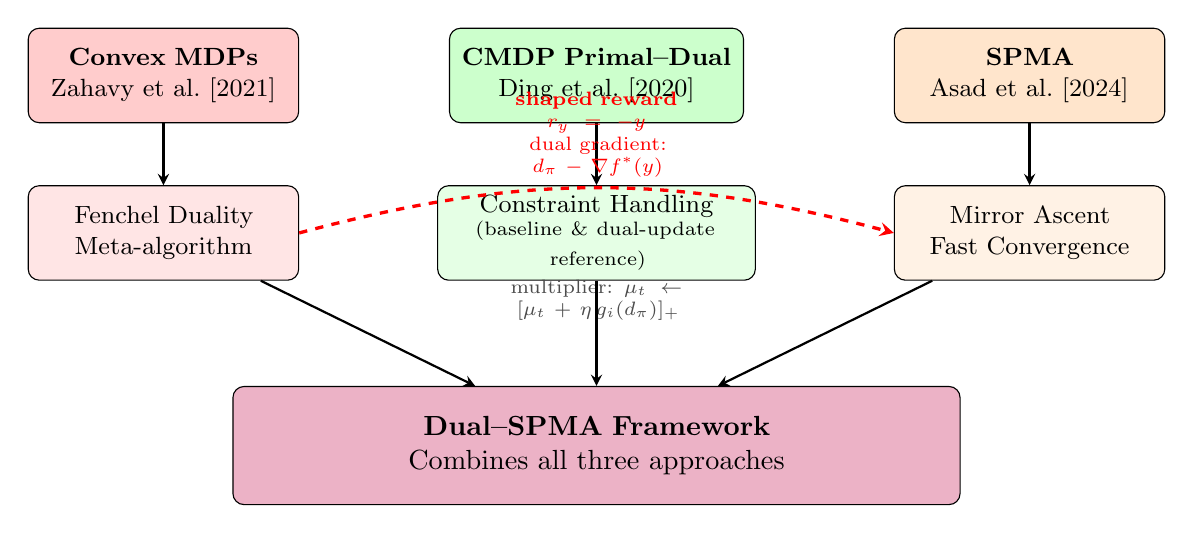
\begin{tikzpicture}[
    block/.style={rectangle, draw, text width=3.2cm, text centered, rounded corners, minimum height=1.2cm, font=\small},
    arrow/.style={->, >=stealth, thick}
]

% ============================================================================
% TOP ROW: Three source papers
% ============================================================================
\node[block, fill=red!20] (paper1) at (0,5) {
    \textbf{Convex MDPs}\\
    Zahavy et al.\ [2021]
};

\node[block, fill=green!20, text width=3.5cm] (paper2) at (5.5,5) {
    \textbf{CMDP Primal--Dual}\\
    Ding et al.\ [2020]
};

\node[block, fill=orange!20] (paper3) at (11,5) {
    \textbf{SPMA}\\
    Asad et al.\ [2024]
};

% ============================================================================
% MIDDLE ROW: Contributions extracted
% ============================================================================
\node[block, fill=red!10] (contrib1) at (0,3) {
    Fenchel Duality\\
    Meta-algorithm
};

\node[block, fill=green!10, text width=3.8cm] (contrib2) at (5.5,3) {
    Constraint Handling\\
    {\scriptsize (baseline \& dual-update\\reference)}
};

\node[block, fill=orange!10] (contrib3) at (11,3) {
    Mirror Ascent\\
    Fast Convergence
};

% Optional: Multiplier update note under middle box (FIX #3)
\node[font=\scriptsize, text width=3.5cm, align=center, text=black!70] (mult) at (5.5,2.15) {
    multiplier: $\mu_t \leftarrow [\mu_t + \eta\, g_i(d_\pi)]_+$
};

% ============================================================================
% BOTTOM ROW: Our framework
% ============================================================================
\node[block, fill=purple!30, text width=9cm, minimum height=1.5cm, font=\normalsize] (ours) at (5.5,0.3) {
    \textbf{Dual--SPMA Framework}\\
    Combines all three approaches
};

% ============================================================================
% ARROWS: Papers to contributions (vertical)
% ============================================================================
\draw[arrow] (paper1) -- (contrib1);
\draw[arrow] (paper2) -- (contrib2);
\draw[arrow] (paper3) -- (contrib3);

% ============================================================================
% Arrow from Convex MDPs to SPMA with annotation
% This shows the shaped reward reduction that connects them
% ============================================================================
\draw[arrow, dashed, red, bend left=15, line width=1.2pt] (contrib1.east) to 
    node[above, font=\scriptsize, text width=2.8cm, align=center] {
        \textbf{shaped reward}\\
        $r_y = -y$\\
        dual gradient:\\
        $d_\pi - \nabla f^*(y)$
    } (contrib3.west);

% ============================================================================
% ARROWS: Contributions to our framework (vertical)
% ============================================================================
\draw[arrow] (contrib1) -- (ours);
\draw[arrow] (contrib2) -- (ours);
\draw[arrow] (contrib3) -- (ours);

\end{tikzpicture}
\caption{%
    \textbf{Overview of the Dual--SPMA framework.} 
    We synthesize ideas from three recent works: (1) the Fenchel duality 
    approach for convex MDPs \citep{zahavy2021reward}, (2) primal-dual 
    methods for constraint handling \citep{ding2020npgpd}, and (3) mirror 
    ascent for fast convergence \citep{asad2024fast}. The key insight is 
    that fixing the dual variable $y$ reduces the policy step to standard 
    RL with shaped reward $r_y = -y$, enabling us to use SPMA as the policy 
    player while Ding et al.\ inform our dual/multiplier updates.
}
\label{fig:framework_overview}
\end{figure}



\textbf{Metrics.} (i) Saddle value $L(\pi,y)$ (when $f^*$ known); (ii) constraint value/violation; (iii) policy return under $r_y$; (iv) convergence of $\|\hat d_{\pi}\|_1$ (tabular) or $\|\widehat{\mathbb E}[\phi]\|$ (FA); (v) wall-clock/sample efficiency. Baselines include NPG--PD.

\small
\bibliographystyle{abbrvnat}
\bibliography{refs}
\end{document}